\documentclass[doc,floatsintext]{apa6}
\usepackage{lmodern}
\usepackage{amssymb,amsmath}
\usepackage{ifxetex,ifluatex}
\usepackage{fixltx2e} % provides \textsubscript
\ifnum 0\ifxetex 1\fi\ifluatex 1\fi=0 % if pdftex
  \usepackage[T1]{fontenc}
  \usepackage[utf8]{inputenc}
\else % if luatex or xelatex
  \ifxetex
    \usepackage{mathspec}
  \else
    \usepackage{fontspec}
  \fi
  \defaultfontfeatures{Ligatures=TeX,Scale=MatchLowercase}
\fi
% use upquote if available, for straight quotes in verbatim environments
\IfFileExists{upquote.sty}{\usepackage{upquote}}{}
% use microtype if available
\IfFileExists{microtype.sty}{%
\usepackage{microtype}
\UseMicrotypeSet[protrusion]{basicmath} % disable protrusion for tt fonts
}{}
\usepackage{hyperref}
\hypersetup{unicode=true,
            pdftitle={Understanding mixed effects models through data simulation},
            pdfauthor={Lisa M. DeBruine~\& Dale J. Barr},
            pdfkeywords={simulation, mixed effects models, power, lme4, R},
            pdfborder={0 0 0},
            breaklinks=true}
\urlstyle{same}  % don't use monospace font for urls
\usepackage{color}
\usepackage{fancyvrb}
\newcommand{\VerbBar}{|}
\newcommand{\VERB}{\Verb[commandchars=\\\{\}]}
\DefineVerbatimEnvironment{Highlighting}{Verbatim}{commandchars=\\\{\}}
% Add ',fontsize=\small' for more characters per line
\usepackage{framed}
\definecolor{shadecolor}{RGB}{248,248,248}
\newenvironment{Shaded}{\begin{snugshade}}{\end{snugshade}}
\newcommand{\AlertTok}[1]{\textcolor[rgb]{0.94,0.16,0.16}{#1}}
\newcommand{\AnnotationTok}[1]{\textcolor[rgb]{0.56,0.35,0.01}{\textbf{\textit{#1}}}}
\newcommand{\AttributeTok}[1]{\textcolor[rgb]{0.77,0.63,0.00}{#1}}
\newcommand{\BaseNTok}[1]{\textcolor[rgb]{0.00,0.00,0.81}{#1}}
\newcommand{\BuiltInTok}[1]{#1}
\newcommand{\CharTok}[1]{\textcolor[rgb]{0.31,0.60,0.02}{#1}}
\newcommand{\CommentTok}[1]{\textcolor[rgb]{0.56,0.35,0.01}{\textit{#1}}}
\newcommand{\CommentVarTok}[1]{\textcolor[rgb]{0.56,0.35,0.01}{\textbf{\textit{#1}}}}
\newcommand{\ConstantTok}[1]{\textcolor[rgb]{0.00,0.00,0.00}{#1}}
\newcommand{\ControlFlowTok}[1]{\textcolor[rgb]{0.13,0.29,0.53}{\textbf{#1}}}
\newcommand{\DataTypeTok}[1]{\textcolor[rgb]{0.13,0.29,0.53}{#1}}
\newcommand{\DecValTok}[1]{\textcolor[rgb]{0.00,0.00,0.81}{#1}}
\newcommand{\DocumentationTok}[1]{\textcolor[rgb]{0.56,0.35,0.01}{\textbf{\textit{#1}}}}
\newcommand{\ErrorTok}[1]{\textcolor[rgb]{0.64,0.00,0.00}{\textbf{#1}}}
\newcommand{\ExtensionTok}[1]{#1}
\newcommand{\FloatTok}[1]{\textcolor[rgb]{0.00,0.00,0.81}{#1}}
\newcommand{\FunctionTok}[1]{\textcolor[rgb]{0.00,0.00,0.00}{#1}}
\newcommand{\ImportTok}[1]{#1}
\newcommand{\InformationTok}[1]{\textcolor[rgb]{0.56,0.35,0.01}{\textbf{\textit{#1}}}}
\newcommand{\KeywordTok}[1]{\textcolor[rgb]{0.13,0.29,0.53}{\textbf{#1}}}
\newcommand{\NormalTok}[1]{#1}
\newcommand{\OperatorTok}[1]{\textcolor[rgb]{0.81,0.36,0.00}{\textbf{#1}}}
\newcommand{\OtherTok}[1]{\textcolor[rgb]{0.56,0.35,0.01}{#1}}
\newcommand{\PreprocessorTok}[1]{\textcolor[rgb]{0.56,0.35,0.01}{\textit{#1}}}
\newcommand{\RegionMarkerTok}[1]{#1}
\newcommand{\SpecialCharTok}[1]{\textcolor[rgb]{0.00,0.00,0.00}{#1}}
\newcommand{\SpecialStringTok}[1]{\textcolor[rgb]{0.31,0.60,0.02}{#1}}
\newcommand{\StringTok}[1]{\textcolor[rgb]{0.31,0.60,0.02}{#1}}
\newcommand{\VariableTok}[1]{\textcolor[rgb]{0.00,0.00,0.00}{#1}}
\newcommand{\VerbatimStringTok}[1]{\textcolor[rgb]{0.31,0.60,0.02}{#1}}
\newcommand{\WarningTok}[1]{\textcolor[rgb]{0.56,0.35,0.01}{\textbf{\textit{#1}}}}
\usepackage{graphicx,grffile}
\makeatletter
\def\maxwidth{\ifdim\Gin@nat@width>\linewidth\linewidth\else\Gin@nat@width\fi}
\def\maxheight{\ifdim\Gin@nat@height>\textheight\textheight\else\Gin@nat@height\fi}
\makeatother
% Scale images if necessary, so that they will not overflow the page
% margins by default, and it is still possible to overwrite the defaults
% using explicit options in \includegraphics[width, height, ...]{}
\setkeys{Gin}{width=\maxwidth,height=\maxheight,keepaspectratio}
\IfFileExists{parskip.sty}{%
\usepackage{parskip}
}{% else
\setlength{\parindent}{0pt}
\setlength{\parskip}{6pt plus 2pt minus 1pt}
}
\setlength{\emergencystretch}{3em}  % prevent overfull lines
\providecommand{\tightlist}{%
  \setlength{\itemsep}{0pt}\setlength{\parskip}{0pt}}
\setcounter{secnumdepth}{0}
% Redefines (sub)paragraphs to behave more like sections
\ifx\paragraph\undefined\else
\let\oldparagraph\paragraph
\renewcommand{\paragraph}[1]{\oldparagraph{#1}\mbox{}}
\fi
\ifx\subparagraph\undefined\else
\let\oldsubparagraph\subparagraph
\renewcommand{\subparagraph}[1]{\oldsubparagraph{#1}\mbox{}}
\fi

%%% Use protect on footnotes to avoid problems with footnotes in titles
\let\rmarkdownfootnote\footnote%
\def\footnote{\protect\rmarkdownfootnote}


  \title{Understanding mixed effects models through data simulation}
    \author{Lisa M. DeBruine\textsuperscript{1}~\& Dale J. Barr\textsuperscript{1}}
    \date{}
  
\shorttitle{Simulating for LMEM}
\affiliation{
\vspace{0.5cm}
\textsuperscript{1} Institute of Neuroscience and Psychology, University of Glasgow}
\keywords{simulation, mixed effects models, power, lme4, R\newline\indent Word count: 5572}
\usepackage{csquotes}
\usepackage{upgreek}
\captionsetup{font=singlespacing,justification=justified}

\usepackage{longtable}
\usepackage{lscape}
\usepackage{multirow}
\usepackage{tabularx}
\usepackage[flushleft]{threeparttable}
\usepackage{threeparttablex}

\newenvironment{lltable}{\begin{landscape}\begin{center}\begin{ThreePartTable}}{\end{ThreePartTable}\end{center}\end{landscape}}

\makeatletter
\newcommand\LastLTentrywidth{1em}
\newlength\longtablewidth
\setlength{\longtablewidth}{1in}
\newcommand{\getlongtablewidth}{\begingroup \ifcsname LT@\roman{LT@tables}\endcsname \global\longtablewidth=0pt \renewcommand{\LT@entry}[2]{\global\advance\longtablewidth by ##2\relax\gdef\LastLTentrywidth{##2}}\@nameuse{LT@\roman{LT@tables}} \fi \endgroup}


\usepackage{lineno}

\linenumbers
\usepackage{float}
\floatplacement{figure}{H}
\raggedbottom
\usepackage{tcolorbox}

\authornote{
Lisa DeBruine 
\includegraphics{images/orcid.png} \url{https://orcid.org/0000-0002-7523-5539}\\
Dale J. Barr 
\includegraphics{images/orcid.png} \url{https://orcid.org/0000-0002-1121-4608}

Correspondence concerning this article should be addressed to Lisa M. DeBruine, 62 Hillhead Street, Glasgow, G12 8QB. E-mail: \href{mailto:lisa.debruine@glasgow.ac.uk}{\nolinkurl{lisa.debruine@glasgow.ac.uk}}}
\note{Preprint submitted for publication}
\abstract{
Experimental designs that sample both subjects and stimuli from a larger population need to account for random effects of both subjects and stimuli using mixed effects models. However, much of this research is analyzed using ANOVA on aggregated responses because researchers are not confident specifying and interpreting mixed effects models. The tutorial will explain how to simulate data with random effects structure and analyse the data using linear mixed effects regression (with the lme4 R package), with a focus on interpreting the output in light of the simulated parameters. Data simulation can not only enhance understanding of how these models work, but also enables researchers to perform power calculations for complex designs. All materials associated with this article can be accessed at \url{https://osf.io/3cz2e/}.



}

\begin{document}
\maketitle

\hypertarget{background}{%
\section{Background}\label{background}}

In this article, we walk through the simulation and analysis of multilevel data with crossed random effects of subjects and stimuli. The article's target audience is researchers who work with experimental designs that sample subjects and stimuli, such as is the case for a large amount of experimental research in face perception, psycholinguistics, or social cognition. The tutorial assumes basic familiarity with R programming.

The R code in this tutorial is supplemented by two web apps at \url{http://shiny.psy.gla.ac.uk/lmem_sim/} and \url{http://shiny.psy.gla.ac.uk/crossed} that perform data simulation without requiring knowledge of R code. These apps allow you to change parameters and inspect the results of LMEM and ANOVA analyses, as well as calculate power and false positive rates for these analyses.

\hypertarget{generalizing-to-a-population-of-encounters}{%
\section{Generalizing to a population of encounters}\label{generalizing-to-a-population-of-encounters}}

Many research questions in psychology and neuroscience are questions about certain types of \emph{events}: What happens when people encounter particular types of stimuli? For example: Do people recognize abstract words faster than concrete words? What impressions do people form about a target person's personality based on their vocal qualities? Can people categorize emotional expressions more quickly on the faces of social ingroup members than on the faces of outgroup members? How do brains respond to threatening versus non-threatening stimuli? In all of these situations, researchers would like to be able to make general statements about phenomena that go beyond the particular participants and particular stimuli that they happen to have chosen for the specific study. Traditionally, people speak of such designs as having \emph{crossed random factors} of participants and stimuli, and have discussed the problem as one of simultaneous generalization to both populations. However, it may be more intuitive to think of the problem as wanting to generalize to a single population of events: in particular, to a population of \emph{encounters} between the units from the sampled populations (Barr, 2018).

Most analyses using conventional statistical techniques, such as analysis of variance and t-test, commit the fallacy of treating stimuli as fixed rather than random. The problem, and the solutions to the problem, have been known in psycholinguistics for over 50 years (Clark, 1973; Coleman, 1964), and most psycholinguistic journals require authors to demonstrate generality of findings over stimuli as well as over subjects. Even so, the quasi-\(F\) statistics for ANOVA (\(F'\) and min-\(F'\)) that Clark proposed as a solution were widely recognized as unreasonably conservative (Forster \& Dickinson, 1976), and until fairly recently, most psycholinguists performed separate by-subjects (\(F_1\)) and by-items analyses (\(F_2\)), declaring an effect \enquote{significant} only if it was significant for both analyses. The \(F_1 \times F_2\) approach was widely used, despite the fact that Clark had already shown it to be invalid, since both \(F\) statistics have higher than nominal false positives in the presence of a null effect, \(F_1\) due to unmodeled stimulus variance, and \(F_2\) due to unmodeled subject variance.

Recently, psycholinguists have adopted linear mixed-effects modeling as the standard for the statistical analysis, given numerous advantages over ANOVA, including the ability to simultaneously model subject and stimulus variation, to gracefully deal with missing data or unbalanced designs, and to accommodate arbitrary types of continuous and categorical predictors or response variables (Baayen, Davidson, \& Bates, 2008; Locker, Hoffman, \& Bovaird, 2007). This development has been facilitated by the \texttt{lme4} package for R (Bates, Mächler, Bolker, \& Walker, 2015), which provides powerful functionality for model specification and estimation. With an appropriately specified model, mixed-effects models yield major improvements in power over quasi-\(F\) approaches and avoid the increased false positive rate associated with separate \(F_1\) and \(F_2\) (Barr et al., 2013).

Despite mixed-effects modeling becoming the \emph{de facto} standard for analysis in psycholinguistics, the approach has yet to take hold in other areas where stimuli are routinely sampled, even in spite of repeated calls for improved analyses in social psychology (Judd, Westfall, \& Kenny, 2012) and neuroimaging (Bedny, Aguirre, \& Thompson-Schill, 2007; Westfall, Nichols, \& Yarkoni, 2016). One of the likely reasons for the limited uptake outside of psycholinguistics is because mixed-effects models expose the analyst to a level of statistical and technical complexity far beyond most researchers' training. While some of this complexity is specific to mixed-effects modeling, some of it is simply hidden away from users of traditional techniques by GUIs and function defaults. The novice mixed modeler is suddenly confronted with the need to make decisions about how to specify categorical predictors, which random effects to include or exclude, which of the statistics in the voluminous output to attend to, and whether and how to re-configure the optimizer function when a convergence error or singularity warning appears.

We are optimisic that the increasing adoption of the mixed-effects approach will improve the generality and thus reproducibility of studies in psychology and related fields, but empathize with the frustration --- and sometimes, exasperation --- expressed by many novices when they attempt to grapple with these models in their research. Much of the uncertainty and unease around mixed-effects models comes from using them in situations where the ground truth is unknown. A profitable way to improve understanding and user confidence is through data simulation. Knowing the ground truth allows the user to experiment with various modeling choices and observe their impact on a model's performance.

\begin{tcolorbox}[colback=black!5!white,colframe=white!5!black,title=Box 1. Glossary of terms]
\begin{longtable}[]{@{}ll@{}}
\begin{minipage}[t]{0.29\columnwidth}\raggedright
crossed random factors\strut
\end{minipage} & \begin{minipage}[t]{0.65\columnwidth}\raggedright
Refers to a design with multiple random factors, such as subjects and items, the levels of which are crossed (e.g., each subject encounters each stimulus) \strut
\end{minipage}\tabularnewline
\begin{minipage}[t]{0.29\columnwidth}\raggedright
data-generating process (DGP)\strut
\end{minipage} & \begin{minipage}[t]{0.65\columnwidth}\raggedright
The mathematical model capturing assumptions about the processes giving rise to the data\strut
\end{minipage}\tabularnewline
\begin{minipage}[t]{0.29\columnwidth}\raggedright
fixed effect\strut
\end{minipage} & \begin{minipage}[t]{0.65\columnwidth}\raggedright
An effect whose value is constant across realizations of the experiment\strut
\end{minipage}\tabularnewline
\begin{minipage}[t]{0.29\columnwidth}\raggedright
random effect\strut
\end{minipage} & \begin{minipage}[t]{0.65\columnwidth}\raggedright
An effect whose value varies across realizations of the experiment (e.g., due to sampling)\strut
\end{minipage}\tabularnewline
\begin{minipage}[t]{0.29\columnwidth}\raggedright
random intercept\strut
\end{minipage} & \begin{minipage}[t]{0.65\columnwidth}\raggedright
A random effect capturing the deviation of a sampling unit (subject or item) from the model intercept\strut
\end{minipage}\tabularnewline
\begin{minipage}[t]{0.29\columnwidth}\raggedright
random slope\strut
\end{minipage} & \begin{minipage}[t]{0.65\columnwidth}\raggedright
A random effect capturing the deviation of a sampling unit (subject or item) from the model slope\strut
\end{minipage}\tabularnewline
\begin{minipage}[t]{0.29\columnwidth}\raggedright
variance components\strut
\end{minipage} & \begin{minipage}[t]{0.65\columnwidth}\raggedright
Parameters describing the distribution of random effects in the
population\strut
\end{minipage}\tabularnewline
\end{longtable}
\end{tcolorbox}

\hypertarget{simulating-data-with-crossed-random-factors}{%
\section{Simulating data with crossed random factors}\label{simulating-data-with-crossed-random-factors}}

To give an overview of the simulation task, we will simulate data from a design with crossed random factors of subjects and stimuli, fit a model to the simulated data, and then try to recover the parameter values we put in from the output. In this hypothetical study, subjects classify the emotional expressions of faces as quickly as possible, and we use their response time as the primary dependent variable. Let's imagine that the faces are of two intrinsic types: either from the subject's ingroup or from an outgroup. For simplicity, we further assume that each face appears only once in the stimulus set. The key question is whether there is any difference in classification speed across the type of face.

\hypertarget{required-software}{%
\subsection{Required software}\label{required-software}}

The simulation will be presented in the R programming language (R Core Team, 2018). To run the code, you will need to have some add-on packages available. Any packages you are missing can be installed using R's \texttt{install.packages()} function, except for the development package \texttt{faux} (DeBruine, 2019) which, at the time of writing, must be installed from the development repository on github.

\begin{Shaded}
\begin{Highlighting}[]
\CommentTok{# load required packages}
\KeywordTok{library}\NormalTok{(}\StringTok{"lme4"}\NormalTok{)        }\CommentTok{# model specification / estimation}
\KeywordTok{library}\NormalTok{(}\StringTok{"afex"}\NormalTok{)        }\CommentTok{# anova and deriving p-values from lmer}
\KeywordTok{library}\NormalTok{(}\StringTok{"broom.mixed"}\NormalTok{) }\CommentTok{# extracting data from model fits }
\KeywordTok{library}\NormalTok{(}\StringTok{"faux"}\NormalTok{)        }\CommentTok{# data simulation}
\CommentTok{# }\AlertTok{NOTE}\CommentTok{: to install the 'faux' package, use:}
\CommentTok{# devtools::install_github("debruine/faux")}
\KeywordTok{library}\NormalTok{(}\StringTok{"tidyverse"}\NormalTok{)   }\CommentTok{# data wrangling and visualisation}
\end{Highlighting}
\end{Shaded}

Because the code uses random number generation, if you want to reproduce the exact results below you will need to set the random number seed at the top of your script and ensure you are using R version 3.6.0 or higher. If you change the seed or are using a lower version of R, your exact numbers will differ, but the procedure will still produce a valid simulation.

\begin{Shaded}
\begin{Highlighting}[]
\CommentTok{# ensure this script returns the same results on each run}
\KeywordTok{set.seed}\NormalTok{(}\DecValTok{8675309}\NormalTok{)}
\end{Highlighting}
\end{Shaded}

\hypertarget{establishing-the-data-generating-parameters}{%
\subsection{Establishing the data-generating parameters}\label{establishing-the-data-generating-parameters}}

The first thing to do is to set up the parameters that govern the process we assume to give rise to the data, the \emph{data-generating process} or DGP. In this hypothetical study, each of 100 subjects will respond to all 50 stimulus items (25 ingroup and 25 outgroup), for a total of 5000 observations.

\hypertarget{specify-the-data-structure}{%
\subsubsection{Specify the data structure}\label{specify-the-data-structure}}

We want the resulting data to be in long format, with the structure shown below, where each row is a single observation for each trial. The variables \texttt{subj\_id} run from \texttt{S001} to \texttt{S100} and index the subject number; \texttt{item\_id} runs from \texttt{I01} to \texttt{I50} and indexes the item number; \texttt{category} says whether the face is ingroup or outgroup, with items 1-25 always ingroup and items 26-50 always outgroup; and \texttt{RT} is the participant's response time for that trial. Note that a trial is uniquely identified by the combination of the \texttt{subj\_id} and \texttt{item\_id} labels.

\begin{table}[H]
\begin{center}
\begin{threeparttable}
\caption{\label{tab:data-example}The target data structure.}
\begin{tabular}{rlllr}
\toprule
row & \multicolumn{1}{c}{subj\_id} & \multicolumn{1}{c}{item\_id} & \multicolumn{1}{c}{category} & \multicolumn{1}{c}{RT}\\
\midrule
1 & S001 & I01 & ingroup & 750.2\\
2 & S001 & I02 & ingroup & 836.1\\
... & ... & ... & ... & ...\\
49 & S001 & I49 & outgroup & 811.9\\
50 & S001 & I50 & outgroup & 801.8\\
51 & S002 & I01 & ingroup & 806.7\\
52 & S002 & I02 & ingroup & 805.9\\
... & ... & ... & ... & ...\\
5000 & S100 & I50 & outgroup & 859.9\\
\bottomrule
\end{tabular}
\end{threeparttable}
\end{center}
\end{table}

Note that for independent variables in designs where subjects and stimuli are crossed, you can't think of factors as being solely \enquote{within} or \enquote{between} because we have two sampling units; you must ask not only whether independent variables are within- or between- subjects, but also whether they are within- or between- stimulus items. Recall that a within-subjects factor is one where each and every subject receives all of the levels, and a between-subjects factors is one where each subject receives only one of the levels. Likewise, a within-items factor is one for which each stimulus receives all of the levels. For our current example, the ingroup/outgroup factor is within subjects but between items, given that each stimulus item is either ingroup or outgroup.

\hypertarget{specify-the-fixed-effects}{%
\subsubsection{Specify the fixed effects}\label{specify-the-fixed-effects}}

Getting an appropriately structured dataset is the easy part. The difficult part is randomly generating the RT values. For this, we need to establish an underlying statistical model. Let us start with a basic model and build up from there. We want a model of RT for subject \(s\) and item \(i\) that looks something like:

\begin{equation}
RT_{si} = \beta_0 + \beta_1 X_{i} + e_{si}.
\end{equation}

\noindent According to the formula, response \(RT_{si}\) for subject \(s\) and item \(i\) is defined as sum of an intercept term \(\beta_0\), which in this example is the grand mean reaction time for the population of stimuli, plus \(\beta_1\), the mean RT difference between ingroup and outgroup stimuli, plus random noise \(e_{si}\). To make \(\beta_0\) equal the grand mean and \(\beta_1\) equal the mean outgroup minus the mean ingroup RT, we will code the \texttt{category} variable as -.5 for the ingroup category and +.5 for the outgroup category.

Although this model is incomplete, we can go ahead and choose parameters for \(\beta_0\) and \(\beta_1\). For this example, we set a grand mean of 800 ms and a mean difference of 50 ms. You will need to use disciplinary expertise and/or pilot data to choose these parameters; by the end of this tutorial you will understand how to extract those parameters from an analysis.

\begin{Shaded}
\begin{Highlighting}[]
\CommentTok{# set fixed effect parameters}
\NormalTok{b0 <-}\StringTok{ }\DecValTok{800} \CommentTok{# intercept; i.e., the grand mean}
\NormalTok{b1 <-}\StringTok{  }\DecValTok{50} \CommentTok{# slope; i.e, effect of category}
\end{Highlighting}
\end{Shaded}

\noindent The parameters \(\beta_0\) and \(\beta_1\) are \emph{fixed effects}: they characterize properties of the population of encounters between subjects and stimuli. Thus, we set the mean RT for a \enquote{typical} subject encountering a \enquote{typical} stimulus to 800 ms, and assume that responses are typically 50 ms slower for outgroup than ingroup faces.

\hypertarget{specify-the-random-effects}{%
\subsubsection{Specify the random effects}\label{specify-the-random-effects}}

This model is completely unrealistic, however, because it doesn't allow for any individual differences among subjects or stimuli. Subjects are not identical in their response characteristics: some will be faster than average, and some slower. We can characterize the difference from the grand mean for each subject \(s\) in terms of a \emph{random effect} \(S_{0s}\), where the first subscript, 0, indicates that the deflection goes with the intercept term, \(\beta_0\). In other words, we assign each subject a unique \emph{random intercept}. Likewise, it is unrealistic to assume that it is equally easy to categorize emotional expressions across all faces in the dataset; some will be easier than others. We incorporate this assumption by including by-item random intercepts \(I_{0i}\), with the subscript 0 reminding us that it is a deflection from the \(\beta_0\) term, and the \(i\) indicating a unique deflection for each of the 50 faces. Adding these terms to our model yields:

\begin{equation}
RT_{si} = \beta_0 + S_{0s} + I_{0i} + \beta_1 X_i + e_{si}
\end{equation}

Now, the actual values for \(S_{0s}\) and \(I_{0i}\) in our sampled dataset will depend on the luck of the draw, i.e., on which subject and which stimuli we happened to have sampled from their respective populations. Unlike fixed effects, we assume these values will differ across different realizations of the experiment. Although the individual values will differ, we assume a fixed standard deviation for the random intercepts in the subject population. Below we assign the by-subject offsets a standard deviation of 100 ms (\texttt{S0s\_sd}), and the by-item offsets a standard deviation of 80 ms (\texttt{I0i\_sd}). We will discuss below how you can estimate these parameters for your own designs.

\begin{Shaded}
\begin{Highlighting}[]
\CommentTok{# set random effect parameters}
\NormalTok{S0s_sd <-}\StringTok{ }\DecValTok{100} \CommentTok{# by-subject random intercept sd}
\NormalTok{I0i_sd <-}\StringTok{  }\DecValTok{80} \CommentTok{# by-item random intercept sd}
\end{Highlighting}
\end{Shaded}

There is still a deficiency in our data-generating model related to \(\beta_1\), the fixed effect of category. Currently our model assumes that each and every subject is exactly 80 ms faster to categorize emotions on ingroup faces than on outgroup faces. Clearly, this assumption is totally unrealistic; some participants will be more sensitive to ingroup/outgroup differences than others. We can capture this in an analogous way to which we captured variation in the intercept, namely by including by-subject \emph{random slopes} \(S_{1s}\).

\begin{equation}
RT_{si} = \beta_0 + S_{0s} + I_{0i} + \left(\beta_1 + S_{1s}\right) X_i + e_{si}
\end{equation}

The random slope \(S_{1s}\) is an estimate of how much faster or slower subject \(s\) is in categorizing ingroup/outgroup faces than the population mean effect \(\beta_1\), which we already set to 50 ms. Given how we coded the \(X_i\) variable, the mean effect for subject \(s\) is given by the \(\beta_1 + S_{1s}\) term. So, a participant who is 90 ms faster on average to categorize ingroup faces would have a random slope \(S_{1s}\) of 40 (\(\beta_1 + S_{1s} = 50 + 40 = 90\)). Likewise, a participant who goes against the grain and shows an effect 15 ms \emph{slower} than average (-15 ms) would have a random slope \(S_{1s}\) of -65 (\(\beta_1 + S_{1s} = 50 + -65 = -15\)). As we did for the random intercepts, we assume that the \(S_{1s}\) effects are the result of sampling, and so will differ across different realizations of the experiment. What remains fixed is their standard deviation \texttt{S1s\_sd}, which we set to 40 ms.

But note that we are sampling \emph{two} random effects for each subject \(s\), a random intercept \(S_{0s}\) and a random slope \(S_{1s}\). It is possible for these values to be correlated, in which case we should not sample them independently. For instance, perhaps people who are faster than average overall (negative random intercept) also show a smaller than average of the ingroup/outgroup manipulation (negative random slope) due to allocating less attention to the task. We can capture this by allowing for a small correlation between the two factors, \texttt{scor}, which we assign to be 0.2.

Finally, we need to characterize the trial-level noise in the study (\(e_{si}\)) in terms of its standard deviation. Here we simply assign this parameter value \texttt{err\_sd} to be twice the size of the by-subject random intercept SD.

\begin{Shaded}
\begin{Highlighting}[]
\CommentTok{# set more random effect and error parameters}
\NormalTok{S1s_sd <-}\StringTok{  }\DecValTok{40} \CommentTok{# by-subject random slope sd}
\NormalTok{scor   <-}\StringTok{  }\FloatTok{.2} \CommentTok{# correlation between intercept and slope}
\NormalTok{err_sd <-}\StringTok{ }\DecValTok{200} \CommentTok{# residual (error) sd}
\end{Highlighting}
\end{Shaded}

To summarize, we established a reasonable statistical model underlying the data having the form:

\begin{equation}
RT_{si} = \beta_0 + S_{0s} + I_{0i} + \left(\beta_1 + S_{1s}\right) X_i + e_{si}
\end{equation}

\noindent The response time for subject \(s\) on item \(i\), \(RT_{si}\), is decomposed into a population grand mean \(\beta_0\), a by-subject random intercept \(S_{0s}\), a by-item random intercept \(I_{0i}\), a fixed slope \(\beta_1\), a by-subject random slope \(S_{1s}\), and a trial-level residual \(e_{si}\). Our data-generating process is fully determined by seven parameters: two fixed effects (intercept \texttt{b0} and slope \texttt{b1}), four variance parameters governing the random effects (\texttt{S0s\_sd}, \texttt{S1s\_sd}, \texttt{scor}, and \texttt{I0i\_sd}), and one parameter governing the trial level variance (\texttt{err\_sd}).

\begin{Shaded}
\begin{Highlighting}[]
\CommentTok{# set all data-generating parameters}
\NormalTok{b0     <-}\StringTok{ }\DecValTok{800} \CommentTok{# intercept; i.e., the grand mean}
\NormalTok{b1     <-}\StringTok{  }\DecValTok{50} \CommentTok{# slope; i.e, effect of category}
\NormalTok{S0s_sd <-}\StringTok{ }\DecValTok{100} \CommentTok{# by-subject random intercept sd}
\NormalTok{I0i_sd <-}\StringTok{  }\DecValTok{80} \CommentTok{# by-item random intercept sd}
\NormalTok{S1s_sd <-}\StringTok{  }\DecValTok{40} \CommentTok{# by-subject random slope sd}
\NormalTok{scor   <-}\StringTok{  }\FloatTok{.2} \CommentTok{# correlation between intercept and slope}
\NormalTok{err_sd <-}\StringTok{ }\DecValTok{200} \CommentTok{# residual (error) sd}
\end{Highlighting}
\end{Shaded}

\noindent In the next section we will apply this data-generating process to simulate the sampling of subjects, items, and trials (encounters).

\hypertarget{simulating-the-sampling-process}{%
\subsection{Simulating the sampling process}\label{simulating-the-sampling-process}}

Let's first define parameters related to the number of observations. In this example, we will simulate data from 100 subjects responding to 25 ingroup faces and 25 outgroup faces. There are no between-subject factors, so we can set \texttt{nsubj} to 100. We set \texttt{nitem} to a named vector specifying the number of items in each between-item group.

\begin{Shaded}
\begin{Highlighting}[]
\CommentTok{# set number of subjects and items}
\NormalTok{nsubj  <-}\StringTok{ }\DecValTok{100} \CommentTok{# number of subjects}
\NormalTok{nitem  <-}\StringTok{ }\KeywordTok{c}\NormalTok{(}\DataTypeTok{ingroup =} \DecValTok{25}\NormalTok{, }\DataTypeTok{outgroup =} \DecValTok{25}\NormalTok{)  }\CommentTok{# number of items}
\end{Highlighting}
\end{Shaded}

\hypertarget{simulate-the-sampling-of-stimulus-items}{%
\subsubsection{Simulate the sampling of stimulus items}\label{simulate-the-sampling-of-stimulus-items}}

We need to create a table listing each item, which category it is in, and simulated values for its random effects. We can do this with the code below, setting item ID to the numbers 1 through the total number of items, category for the first 25 items to \enquote{ingroup} and the next 25 faces to \enquote{outgroup}, and sampling 50 numbers from a normal distribution with a mean of 0 and a standard deviation of \texttt{I0i\_sd}.

\begin{Shaded}
\begin{Highlighting}[]
\CommentTok{# simulate a sample of items}
\NormalTok{items <-}\StringTok{ }\KeywordTok{data.frame}\NormalTok{(}
  \DataTypeTok{item_id =} \DecValTok{1}\OperatorTok{:}\KeywordTok{sum}\NormalTok{(nitem),}
  \DataTypeTok{category =} \KeywordTok{rep}\NormalTok{(}\KeywordTok{c}\NormalTok{(}\StringTok{"ingroup"}\NormalTok{, }\StringTok{"outgroup"}\NormalTok{), nitem),}
  \DataTypeTok{I0i =} \KeywordTok{rnorm}\NormalTok{(}\KeywordTok{sum}\NormalTok{(nitem), }\DecValTok{0}\NormalTok{, I0i_sd)}
\NormalTok{)}
\end{Highlighting}
\end{Shaded}

The function \texttt{faux::sim\_design()} is a more flexible way to generate data with specified parameters. This function will create a dataset with any number of between and/or within factors, \texttt{n} items per between-cell, and the specified means (\texttt{mu}), standard deviations (\texttt{sd}) and correlations (\texttt{r}). By default, it plots a schematic of the design you specified. See the package vignette (DeBruine, 2019) for more details.

Category is a between-items factor, so we need to include it in the \texttt{between} argument. Set \texttt{n\ =\ nitem} to specify the number of items per category. Set \texttt{sd\ =\ I0i\_sd} to set the standard deviation for the by-item random effects. Set \texttt{dv\ =\ "I0i"} to give the random effect column that name. Set \texttt{id\ =\ "item\_id"}; we'll use this later to join this information to the table of trials.

\begin{Shaded}
\begin{Highlighting}[]
\CommentTok{# simulate a sample of items using sim_design()}
\NormalTok{items <-}\StringTok{ }\NormalTok{faux}\OperatorTok{::}\KeywordTok{sim_design}\NormalTok{(}
  \DataTypeTok{between =} \KeywordTok{list}\NormalTok{(}\DataTypeTok{category =} \KeywordTok{c}\NormalTok{(}\StringTok{"ingroup"}\NormalTok{, }\StringTok{"outgroup"}\NormalTok{)),}
  \DataTypeTok{n =}\NormalTok{ nitem,}
  \DataTypeTok{sd =}\NormalTok{ I0i_sd,}
  \DataTypeTok{dv =} \StringTok{"I0i"}\NormalTok{,}
  \DataTypeTok{id =} \StringTok{"item_id"}
\NormalTok{)}
\end{Highlighting}
\end{Shaded}

\begin{figure}

{\centering 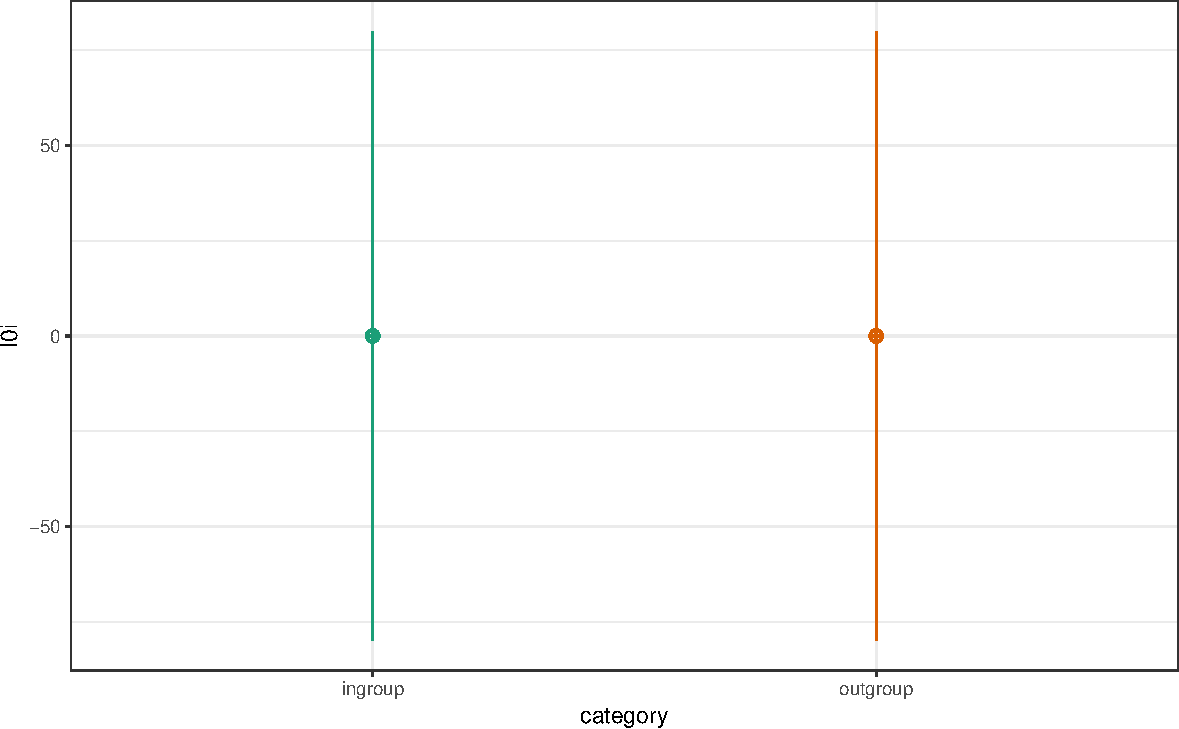
\includegraphics[width=0.75\linewidth]{images/sim-items-1} 

}

\caption{The specified distribution of random effects for ingroup and outgroup faces.}\label{fig:sim-items}
\end{figure}

We will also introduce a numerical predictor to represent what category each stimulus item \(i\) appears in (i.e., for the \(X_i\) in our model). Since we predict that responses to ingroup faces will be faster than outgroup faces, we set ingroup to -0.5 and outgroup to +0.5. We will later multiply this \emph{effect coded} factor by the fixed effect of category (\texttt{b1} = 50) to simulate data where the ingroup faces are on average -25 ms different from the grand mean, while the outgroup faces are on average 25 ms different from the grand mean.

\begin{Shaded}
\begin{Highlighting}[]
\CommentTok{# effect-code category}
\NormalTok{items}\OperatorTok{$}\NormalTok{cat <-}\StringTok{ }\KeywordTok{recode}\NormalTok{(items}\OperatorTok{$}\NormalTok{category, }\StringTok{"ingroup"}\NormalTok{ =}\StringTok{ }\FloatTok{-0.5}\NormalTok{, }\StringTok{"outgroup"}\NormalTok{ =}\StringTok{ }\FloatTok{+0.5}\NormalTok{)}
\end{Highlighting}
\end{Shaded}

\begin{table}[H]
\begin{center}
\begin{threeparttable}
\caption{\label{tab:items-table}The resulting table of item parameters.}
\begin{tabular}{llrrllrrllrrllrr}
\toprule
item\_id & \multicolumn{1}{c}{category} & \multicolumn{1}{c}{I0i} & \multicolumn{1}{c}{cat}\\
\midrule
S01 & ingroup & 59.6 & -0.5\\
S02 & ingroup & -107.7 & -0.5\\
S03 & ingroup & 26.4 & -0.5\\
S04 & ingroup & -1.0 & -0.5\\
S05 & ingroup & -37.1 & -0.5\\
S06 & ingroup & 16.4 & -0.5\\
\bottomrule
\end{tabular}
\end{threeparttable}
\end{center}
\end{table}

\hypertarget{simulate-the-sampling-of-subjects}{%
\subsubsection{Simulate the sampling of subjects}\label{simulate-the-sampling-of-subjects}}

Now we will simulate the sampling of individual subjects, resulting in a table listing each subject and their two correlated random effects. We will again use \texttt{faux::sim\_design()} for this task.

Set the \texttt{within} argument in \texttt{sim\_design()} to a list with one factor (\texttt{effect}) that has two levels: \texttt{S0s} and \texttt{S1s}. If you set a factor's levels as a named vector, the names (\texttt{S0s} and \texttt{S1s}) become the column names in the data table and the values are used in plots created by faux.

Set \texttt{n\ =\ nsubj} to specify the number of subjects. There are two random effects to specify standard deviation for, so set \texttt{sd} using a named vector and set their correlation with \texttt{r = scor}. Set \texttt{id\ =\ "subj\_id"}; we'll use this later to join this information to the table of trials.

\begin{Shaded}
\begin{Highlighting}[]
\CommentTok{# simulate a sample of subjects}
\NormalTok{subjects <-}\StringTok{ }\NormalTok{faux}\OperatorTok{::}\KeywordTok{sim_design}\NormalTok{(}
  \DataTypeTok{within =} \KeywordTok{list}\NormalTok{(}\DataTypeTok{effect =} \KeywordTok{c}\NormalTok{(}\DataTypeTok{S0s =} \StringTok{"By-subject random intercepts"}\NormalTok{, }
                           \DataTypeTok{S1s =} \StringTok{"By-subject random slopes"}\NormalTok{)), }
  \DataTypeTok{n =}\NormalTok{ nsubj,}
  \DataTypeTok{sd =} \KeywordTok{c}\NormalTok{(S0s_sd, S1s_sd), }
  \DataTypeTok{r =}\NormalTok{ scor,}
  \DataTypeTok{id =} \StringTok{"subj_id"}
\NormalTok{)}
\end{Highlighting}
\end{Shaded}

\begin{figure}

{\centering 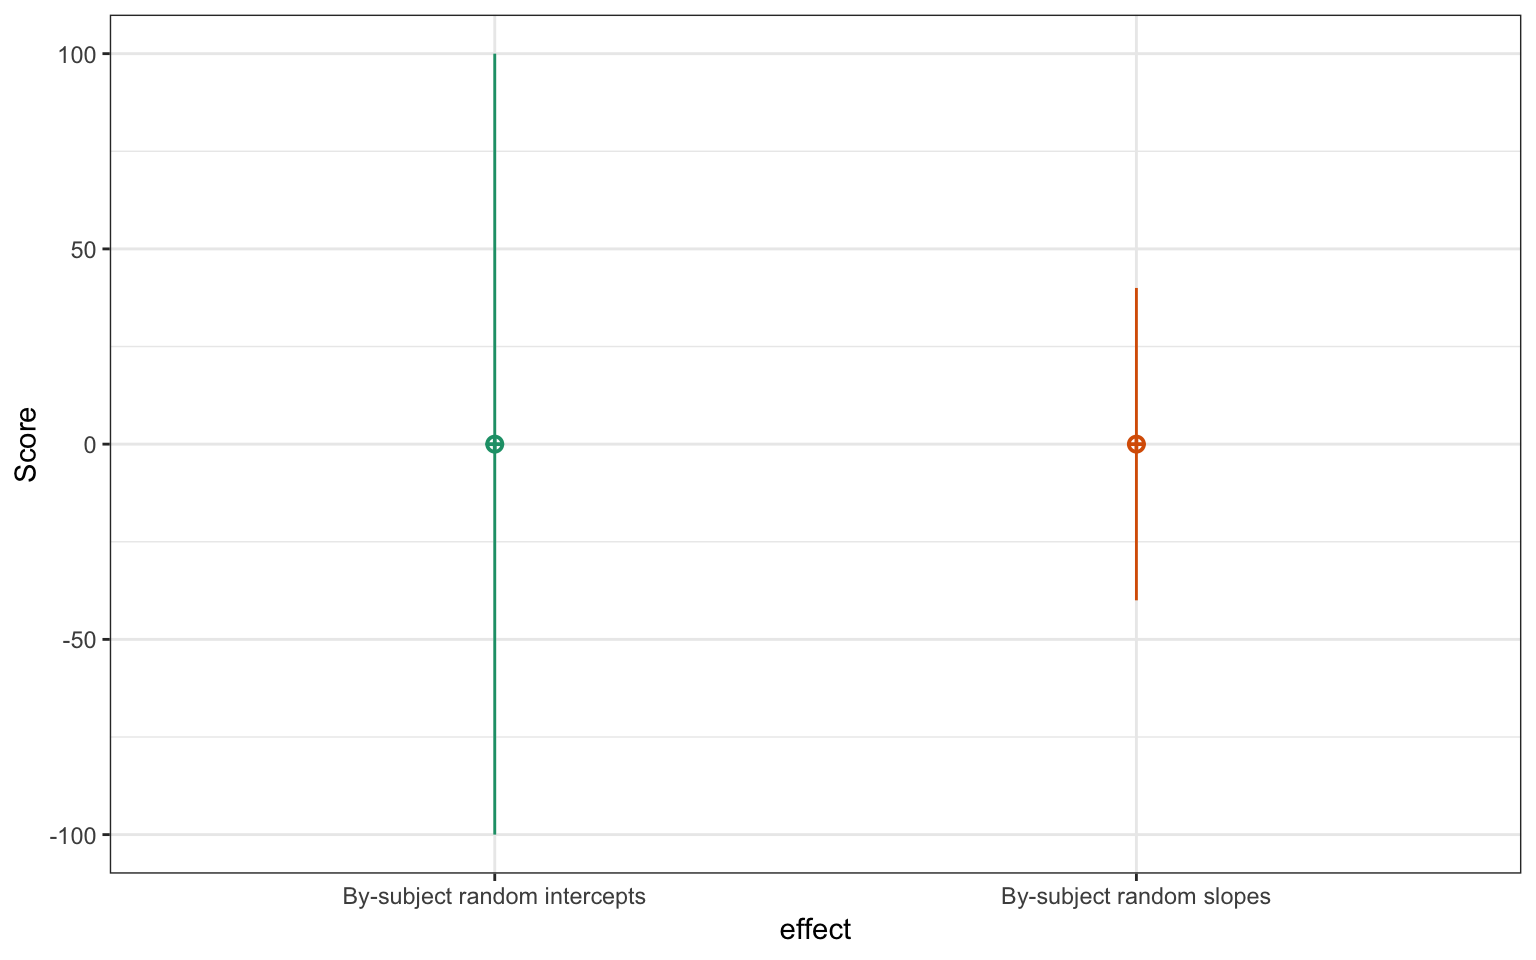
\includegraphics[width=0.75\linewidth]{images/sim-subjects-1} 

}

\caption{The specified distribution of random effects for subjects}\label{fig:sim-subjects}
\end{figure}

\begin{table}[H]
\begin{center}
\begin{threeparttable}
\caption{\label{tab:subj-table}The resulting table of subject parameters.}
\begin{tabular}{lll}
\toprule
subj\_id & \multicolumn{1}{c}{S0s} & \multicolumn{1}{c}{S1s}\\
\midrule
S001 & -98.77 & -49.49\\
S002 & 37.33 & 23.77\\
S003 & -127.42 & 39.56\\
S004 & -56.37 & 10.13\\
S005 & -39.73 & -8.05\\
S006 & 43.70 & 37.66\\
\bottomrule
\end{tabular}
\end{threeparttable}
\end{center}
\end{table}

\hypertarget{simulate-trials-encounters}{%
\subsubsection{Simulate trials (encounters)}\label{simulate-trials-encounters}}

Since all subjects respond to all items, we can set up a table of trials by making every possible combination of the subject and item IDs using the function \texttt{crossing()} from tidyr (Wickham \& Henry, 2019). Once we have a table of all trials, we can join the information in this table to the information in our \texttt{subjects} and \texttt{items} tables using \texttt{dplyr::inner\_join()}. Each trial has random error associated; we simulate this from a normal distribution with a mean of 0 and SD of \texttt{err\_sd}.

\begin{Shaded}
\begin{Highlighting}[]
\CommentTok{# cross subject and item IDs; add an error term}
\NormalTok{trials <-}\StringTok{ }\KeywordTok{crossing}\NormalTok{(}\DataTypeTok{subj_id =}\NormalTok{ subjects}\OperatorTok{$}\NormalTok{subj_id,}
                   \DataTypeTok{item_id =}\NormalTok{ items}\OperatorTok{$}\NormalTok{item_id)  }\OperatorTok
\StringTok{  }\KeywordTok{mutate}\NormalTok{(}\DataTypeTok{err =} \KeywordTok{rnorm}\NormalTok{(}\KeywordTok{nrow}\NormalTok{(.), }\DataTypeTok{mean =} \DecValTok{0}\NormalTok{, }\DataTypeTok{sd =}\NormalTok{ err_sd))}

\CommentTok{# join subject and item tables}
\NormalTok{joined <-}\StringTok{ }\NormalTok{trials }\OperatorTok
\StringTok{  }\KeywordTok{inner_join}\NormalTok{(subjects, }\StringTok{"subj_id"}\NormalTok{) }\OperatorTok
\StringTok{  }\KeywordTok{inner_join}\NormalTok{(items, }\StringTok{"item_id"}\NormalTok{)}
\end{Highlighting}
\end{Shaded}

\begin{table}[H]
\begin{center}
\begin{threeparttable}
\caption{\label{tab:trials-table}The resulting table of trials joined to the subject and item tables.}
\begin{tabular}{llrrrlrrllrrrlrrllrrrlrrllrrrlrrllrrrlrrllrrrlrrllrrrlrrllrrrlrr}
\toprule
subj\_id & \multicolumn{1}{c}{item\_id} & \multicolumn{1}{c}{err} & \multicolumn{1}{c}{S0s} & \multicolumn{1}{c}{S1s} & \multicolumn{1}{c}{category} & \multicolumn{1}{c}{I0i} & \multicolumn{1}{c}{cat}\\
\midrule
S001 & S01 & 308.0 & -98.8 & -49.5 & ingroup & 59.6 & -0.5\\
S001 & S02 & 85.3 & -98.8 & -49.5 & ingroup & -107.7 & -0.5\\
S001 & S03 & -205.3 & -98.8 & -49.5 & ingroup & 26.4 & -0.5\\
S001 & S04 & -138.1 & -98.8 & -49.5 & ingroup & -1.0 & -0.5\\
S001 & S05 & -190.8 & -98.8 & -49.5 & ingroup & -37.1 & -0.5\\
S001 & S06 & -351.1 & -98.8 & -49.5 & ingroup & 16.4 & -0.5\\
\bottomrule
\end{tabular}
\end{threeparttable}
\end{center}
\end{table}

\hypertarget{calculate-the-response-values}{%
\subsubsection{Calculate the response values}\label{calculate-the-response-values}}

Note how this resulting table contains the full decomposition of effects that we need to compute the response according to the linear model we defined above:

\begin{equation}
RT_{si} = \beta_0 + S_{0s} + I_{0i} + \left(\beta_1 + S_{1s}\right) X_i + e_{si}
\end{equation}

Thus, we will calculate the response variable \texttt{RT} by adding together:

\begin{itemize}
\tightlist
\item
  the grand intercept (\texttt{b0}),
\item
  each subject-specific random intercept (\texttt{S0s}),
\item
  each item-specific random intercept (\texttt{I0i}),
\item
  each sum of the category effect (\texttt{b1}) and the random slope (\texttt{S1s}), multiplied by the numerical predictor (\texttt{cat}), and
\item
  each residual error (\texttt{err}).
\end{itemize}

After this we will use \texttt{dplyr::select()} to keep the columns we need. Note that the resulting table has the structure that we set as our goal at the start of this exercise, with the additional column \texttt{cat}, which we will keep to use in the estimation process, described in the next section.

\begin{Shaded}
\begin{Highlighting}[]
\CommentTok{# calculate the response variable}
\NormalTok{dat_sim <-}\StringTok{ }\NormalTok{joined }\OperatorTok
\StringTok{  }\KeywordTok{mutate}\NormalTok{(}\DataTypeTok{RT =}\NormalTok{ b0 }\OperatorTok{+}\StringTok{ }\NormalTok{I0i }\OperatorTok{+}\StringTok{ }\NormalTok{S0s }\OperatorTok{+}\StringTok{ }\NormalTok{(b1 }\OperatorTok{+}\StringTok{ }\NormalTok{S1s) }\OperatorTok{*}\StringTok{ }\NormalTok{cat }\OperatorTok{+}\StringTok{ }\NormalTok{err) }\OperatorTok
\StringTok{  }\KeywordTok{select}\NormalTok{(subj_id, item_id, category, cat, RT)}
\end{Highlighting}
\end{Shaded}

\begin{table}[H]
\begin{center}
\begin{threeparttable}
\caption{\label{tab:dat-sim-table}The final simulated dataset.}
\begin{tabular}{lllrrlllrrlllrrlllrrlllrr}
\toprule
subj\_id & \multicolumn{1}{c}{item\_id} & \multicolumn{1}{c}{category} & \multicolumn{1}{c}{cat} & \multicolumn{1}{c}{RT}\\
\midrule
S001 & S01 & ingroup & -0.5 & 1,068.5\\
S001 & S02 & ingroup & -0.5 & 678.6\\
S001 & S03 & ingroup & -0.5 & 522.1\\
S001 & S04 & ingroup & -0.5 & 561.9\\
S001 & S05 & ingroup & -0.5 & 473.1\\
S001 & S06 & ingroup & -0.5 & 366.2\\
\bottomrule
\end{tabular}
\end{threeparttable}
\end{center}
\end{table}

\hypertarget{data-simulation-function}{%
\subsubsection{Data simulation function}\label{data-simulation-function}}

To make it easier to try out different parameters or to generate many datasets for the purpose of power analysis, you can put all of the code above into a custom function. Set up the function to takes all of the parameters we set above as arguments. We'll set the defaults to the values we used, but you can choose your own defaults. The code below is just all of the code above, condensed a bit. It returns one dataset with the parameters you specified.

\begin{Shaded}
\begin{Highlighting}[]
\CommentTok{# set up the custom data simulation function}
\NormalTok{my_sim_data <-}\StringTok{ }\ControlFlowTok{function}\NormalTok{(}
  \DataTypeTok{nsubj  =} \DecValTok{100}\NormalTok{, }\CommentTok{# number of subjects}
  \DataTypeTok{nitem  =} \KeywordTok{c}\NormalTok{(}\DataTypeTok{ingroup =} \DecValTok{25}\NormalTok{, }\DataTypeTok{outgroup =} \DecValTok{25}\NormalTok{),  }\CommentTok{# number of items}
  \DataTypeTok{b0     =} \DecValTok{800}\NormalTok{, }\CommentTok{# grand mean}
  \DataTypeTok{b1     =}  \DecValTok{50}\NormalTok{, }\CommentTok{# effect of category}
  \DataTypeTok{I0i_sd =}  \DecValTok{80}\NormalTok{, }\CommentTok{# by-item random intercept sd}
  \DataTypeTok{S0s_sd =} \DecValTok{100}\NormalTok{, }\CommentTok{# by-subject random intercept sd}
  \DataTypeTok{S1s_sd =}  \DecValTok{40}\NormalTok{, }\CommentTok{# by-subject random slope sd}
  \DataTypeTok{scor   =} \FloatTok{0.2}\NormalTok{, }\CommentTok{# correlation between intercept and slope}
  \DataTypeTok{err_sd =} \DecValTok{200}\NormalTok{)\{  }\CommentTok{# residual (standard deviation)}
  
  \CommentTok{# simulate items}
\NormalTok{  items <-}\StringTok{ }\NormalTok{faux}\OperatorTok{::}\KeywordTok{sim_design}\NormalTok{(}
    \DataTypeTok{between =} \KeywordTok{list}\NormalTok{(}\DataTypeTok{category =} \KeywordTok{c}\NormalTok{(}\StringTok{"ingroup"}\NormalTok{, }\StringTok{"outgroup"}\NormalTok{)),}
    \DataTypeTok{n =}\NormalTok{ nitem,}
    \DataTypeTok{sd =}\NormalTok{ I0i_sd,}
    \DataTypeTok{dv =} \StringTok{"I0i"}\NormalTok{,}
    \DataTypeTok{id =} \StringTok{"item_id"}\NormalTok{,}
    \DataTypeTok{plot =} \OtherTok{FALSE}
\NormalTok{  )}

  \CommentTok{# effect code category}
\NormalTok{  items}\OperatorTok{$}\NormalTok{cat <-}\StringTok{ }\KeywordTok{recode}\NormalTok{(items}\OperatorTok{$}\NormalTok{category, }\StringTok{"ingroup"}\NormalTok{ =}\StringTok{ }\FloatTok{-0.5}\NormalTok{, }\StringTok{"outgroup"}\NormalTok{ =}\StringTok{ }\FloatTok{0.5}\NormalTok{)}
  
  \CommentTok{# simulate subjects}
\NormalTok{  subjects <-}\StringTok{ }\NormalTok{faux}\OperatorTok{::}\KeywordTok{sim_design}\NormalTok{(}
    \DataTypeTok{within =} \KeywordTok{list}\NormalTok{(}\DataTypeTok{effect =} \KeywordTok{c}\NormalTok{(}\DataTypeTok{S0s =} \StringTok{"By-subject random intercepts"}\NormalTok{, }
                             \DataTypeTok{S1s =} \StringTok{"By-subject random slopes"}\NormalTok{)), }
    \DataTypeTok{n =}\NormalTok{ nsubj,}
    \DataTypeTok{sd =} \KeywordTok{c}\NormalTok{(S0s_sd, S1s_sd), }
    \DataTypeTok{r =}\NormalTok{ scor,}
    \DataTypeTok{id =} \StringTok{"subj_id"}\NormalTok{,}
    \DataTypeTok{plot =} \OtherTok{FALSE}
\NormalTok{  )}
  
  \CommentTok{# simulate trials}
\NormalTok{  dat_sim <-}\StringTok{ }\KeywordTok{crossing}\NormalTok{(}\DataTypeTok{subj_id =}\NormalTok{ subjects}\OperatorTok{$}\NormalTok{subj_id,}
                      \DataTypeTok{item_id =}\NormalTok{ items}\OperatorTok{$}\NormalTok{item_id) }\OperatorTok
\StringTok{    }\KeywordTok{inner_join}\NormalTok{(subjects, }\StringTok{"subj_id"}\NormalTok{) }\OperatorTok
\StringTok{    }\KeywordTok{inner_join}\NormalTok{(items, }\StringTok{"item_id"}\NormalTok{) }\OperatorTok
\StringTok{    }\KeywordTok{mutate}\NormalTok{(}\DataTypeTok{err =} \KeywordTok{rnorm}\NormalTok{(}\KeywordTok{nrow}\NormalTok{(.), }\DataTypeTok{mean =} \DecValTok{0}\NormalTok{, }\DataTypeTok{sd =}\NormalTok{ err_sd)) }\OperatorTok
\StringTok{    }\KeywordTok{mutate}\NormalTok{(}\DataTypeTok{RT =}\NormalTok{ b0 }\OperatorTok{+}\StringTok{ }\NormalTok{I0i }\OperatorTok{+}\StringTok{ }\NormalTok{S0s }\OperatorTok{+}\StringTok{ }\NormalTok{(b1 }\OperatorTok{+}\StringTok{ }\NormalTok{S1s) }\OperatorTok{*}\StringTok{ }\NormalTok{cat }\OperatorTok{+}\StringTok{ }\NormalTok{err) }\OperatorTok
\StringTok{    }\KeywordTok{select}\NormalTok{(subj_id, item_id, category, cat, RT)}
  
\NormalTok{  dat_sim}
\NormalTok{\}}
\end{Highlighting}
\end{Shaded}

Now you can generate a dataset with the default parameters using \texttt{my\_sim\_data()} or, for example, a dataset with 500 subjects and no effect of category using \texttt{my\_sim\_data(nsubj\ =\ 50,\ b1\ =\ 0)}.

\hypertarget{analyzing-the-simulated-data}{%
\section{Analyzing the simulated data}\label{analyzing-the-simulated-data}}

\hypertarget{setting-up-the-formula}{%
\subsection{Setting up the formula}\label{setting-up-the-formula}}

Now we're ready to analyse our simulated data. The first argument to \texttt{lmer()} is a model formula that defines the structure of the linear model. The formula for our design maps onto how we calculated the response above.

\begin{verbatim}
RT ~ 1 + cat + (1 | item_id) + (1 + cat | subj_id)
\end{verbatim}

\begin{itemize}
\tightlist
\item
  \texttt{RT} is the response
\item
  \texttt{1} corresponds to the grand intercept (\texttt{b0}),
\item
  \texttt{cat} corresponds to the effect of category (\texttt{b1\ *\ cat}),
\item
  \texttt{(1\ \textbar{}\ item\_id)} corresponds to the item-specific random intercept (\texttt{I0i}),
\item
  \texttt{(1\ +\ cat\ \textbar{}\ subj\_id)} corresponds to the subject-specific random intercept (\texttt{S0s}) plus the subject-specific random slope of category (\texttt{S1s}),
\item
  the error term is automatically included in all models, so is left implicit
\end{itemize}

The \enquote{fixed} part of the formula, \texttt{RT\ \textasciitilde{}\ 1\ +\ cat}, establishes the \(RT_{si} + \beta_0 + \beta_1 X_i + e_{si}\) part of our linear model, with the role of \(X_i\) being played by \texttt{cat}. Every model has an intercept (\(\beta_0\)) term and residual term (\(e_{si}\)) by default, so you could alternatively leave the \texttt{1} out and just write \texttt{RT\ \textasciitilde{}\ cat}.

The terms in parentheses with the \texttt{\textbar{}} separator define the random effects structure. For each of these bracketed terms, the left-hand side of the \texttt{\textbar{}} names the effects you wish to allow to vary and the right hand side names the variable identifying the levels of the random factor over which the terms vary (e.g., subjects or items). The first term, \texttt{(1\ \textbar{}\ item\_id)} allows the intercept (\texttt{1}) to vary over the random factor of items (\texttt{item\_id}). This is an instruction to estimate the parameter underlying the \texttt{I0i} values, namely \texttt{I0i\_sd}. The second term, \texttt{(1\ +\ cat\ \textbar{}\ subj\_id)}, allows both the intercept and the effect of category (\texttt{cat}) to vary over the random factor of subjects (\texttt{subj\_id}). It is an instruction to estimate the three parameters that underlie the \texttt{S0s} and \texttt{S1s} values, namely \texttt{S0s\_sd}, \texttt{S1s\_sd}, and \texttt{scor}.

\hypertarget{interpreting-the-lmer-summary}{%
\subsection{Interpreting the lmer summary}\label{interpreting-the-lmer-summary}}

The other arguments to the \texttt{lme4} function are the name of the data frame where the values are found (\texttt{dat\_sim}), and \texttt{REML\ =\ FALSE} which selects maximum-likelihood estimation, which is preferable to the default estimation technique when testing fixed effects. Use the \texttt{summary()} function to view the results.

\begin{Shaded}
\begin{Highlighting}[]
\CommentTok{# fit a linear mixed-effects model to data}
\NormalTok{mod_sim <-}\StringTok{ }\KeywordTok{lmer}\NormalTok{(RT }\OperatorTok{~}\StringTok{ }\DecValTok{1} \OperatorTok{+}\StringTok{ }\NormalTok{cat }\OperatorTok{+}\StringTok{ }\NormalTok{(}\DecValTok{1} \OperatorTok{|}\StringTok{ }\NormalTok{item_id) }\OperatorTok{+}\StringTok{ }\NormalTok{(}\DecValTok{1} \OperatorTok{+}\StringTok{ }\NormalTok{cat }\OperatorTok{|}\StringTok{ }\NormalTok{subj_id),}
                \DataTypeTok{data =}\NormalTok{ dat_sim, }\DataTypeTok{REML =} \OtherTok{FALSE}\NormalTok{)}

\KeywordTok{summary}\NormalTok{(mod_sim, }\DataTypeTok{corr =} \OtherTok{FALSE}\NormalTok{)}
\end{Highlighting}
\end{Shaded}

\begin{verbatim}
## Linear mixed model fit by maximum likelihood . t-tests use
##   Satterthwaite's method [lmerModLmerTest]
## Formula: RT ~ 1 + cat + (1 | item_id) + (1 + cat | subj_id)
##    Data: dat_sim
## 
##      AIC      BIC   logLik deviance df.resid 
##  67720.6  67766.2 -33853.3  67706.6     4993 
## 
## Scaled residuals: 
##     Min      1Q  Median      3Q     Max 
## -3.7631 -0.6740 -0.0046  0.6778  3.6425 
## 
## Random effects:
##  Groups   Name        Variance Std.Dev. Corr
##  subj_id  (Intercept) 10334    101.66       
##           cat          2413     49.12   0.16
##  item_id  (Intercept)  4574     67.63       
##  Residual             40770    201.92       
## Number of obs: 5000, groups:  subj_id, 100; item_id, 50
## 
## Fixed effects:
##             Estimate Std. Error     df t value Pr(>|t|)    
## (Intercept)   816.05      14.25 126.62   57.28   <2e-16 ***
## cat            52.42      20.56  55.35    2.55   0.0136 *  
## ---
## Signif. codes:  0 '***' 0.001 '**' 0.01 '*' 0.05 '.' 0.1 ' ' 1
\end{verbatim}

\noindent Let's break down the output step-by-step and try to find estimates of the seven parameters we used to generate the data: \texttt{b0}, \texttt{b1}, \texttt{S0s\_sd}, \texttt{S1s\_sd}, \texttt{scor}, \texttt{I0i\_sd} and \texttt{err}. If you analyze existing data with a mixed effects model, you can use these estimates to help you set reasonable values for random effects in your own simulations.

After providing general information about the model fit, the output is divided into a \texttt{Random\ effects} and a \texttt{Fixed\ effects} section. The fixed effects section should be familiar from other types of linear models.

\begin{verbatim}
## Fixed effects:
##             Estimate Std. Error     df t value Pr(>|t|)    
## (Intercept)   816.05      14.25 126.62   57.28   <2e-16 ***
## cat            52.42      20.56  55.35    2.55   0.0136 *
\end{verbatim}

\noindent The \texttt{Estimate} column gives us parameter estimates for the fixed effects in the model, i.e., \(\hat{\beta_0}\) and \(\hat{\beta_1}\), which are estimated at about 816.05 and 52.42. The next columns give us the standard errors, estimated degrees of freedom (using the Satterthwaite approach), \(t\) value, and finally, \(p\) value.

The \texttt{Random\ effects} section is specific to mixed-effects models, and will be less familiar to the reader.

\begin{verbatim}
## Random effects:
##  Groups   Name        Variance Std.Dev. Corr
##  subj_id  (Intercept) 10334    101.66       
##           cat          2413     49.12   0.16
##  item_id  (Intercept)  4574     67.63       
##  Residual             40770    201.92
\end{verbatim}

\noindent These are the estimates for the \emph{variance components} in the model. To avoid confusion, it is best to think of the information in this table as coming from three separate tables divided up by the values in the \texttt{Groups} column.

The first subtable, where the value of \texttt{Groups} is \texttt{subj\_id}, gives the estimates for the variance parameters defining the by-subject random effects.

\begin{verbatim}
##  Groups   Name        Variance Std.Dev. Corr
##  subj_id  (Intercept) 10334    101.66       
##           cat          2413     49.12   0.16
\end{verbatim}

\noindent We have estimates for the variance of the intercept and slope (\texttt{cat}) in the \texttt{Variance} column, which is just the square of the standard deviation in the \texttt{Std.Dev.} column. We obtain estimates for \texttt{S0s\_sd} and \texttt{S1s\_sd} of 101.66 and 49.12 respectively. The \texttt{Corr.} column gives us the estimated correlation between the by-subject random intercepts and slopes, estimated here as 0.16.

The second subtable gives us the by-item random effect parameter estimates of which there is only one, 67.63, corresponding to \texttt{I0i\_sd}. Again, the \texttt{Variance} column is just this value squared.

\begin{verbatim}
##  Groups   Name        Variance Std.Dev. Corr
##  item_id  (Intercept)  4574     67.63
\end{verbatim}

The last subtable gives us the estimate of the residual term, 201.92.

\begin{verbatim}
##  Groups   Name        Variance Std.Dev. Corr
##  Residual             40770    201.92
\end{verbatim}

We have found all seven parameters in the output. Let's compare them to the values that we put in.

\begin{table}[H]
\begin{center}
\begin{threeparttable}
\caption{\label{tab:param-compare}The simulation parameters compared to the model estimations.}
\begin{tabular}{llrrllrrllrrllrr}
\toprule
variable & \multicolumn{1}{c}{explanation} & \multicolumn{1}{c}{simulated value} & \multicolumn{1}{c}{estimated by model}\\
\midrule
b0 & intercept (grand mean) & 800.0 & 816.05\\
b1 & fixed effect of category & 50.0 & 52.42\\
S0s\_sd & by-subject random intercept SD & 100.0 & 101.66\\
S1s\_sd & by-subject random slope SD & 40.0 & 49.12\\
scor & cor between intercept and slope & 0.2 & 0.16\\
I0i\_sd & by-item random intercept SD & 80.0 & 67.63\\
err\_sd & residual (error) SD & 200.0 & 201.92\\
\bottomrule
\end{tabular}
\end{threeparttable}
\end{center}
\end{table}

You can also use \texttt{broom.mixed::tidy()} to output fixed and/or random effects in a tidy table. This is especially useful when you need to combine the output from hundreds of simulations to calculate power. The code below adds a column with the simulated parameters we set above so you can compare them to the estimated parameters from this simulated dataset.

\begin{Shaded}
\begin{Highlighting}[]
\CommentTok{# get a tidy table of results}
\NormalTok{broom.mixed}\OperatorTok{::}\KeywordTok{tidy}\NormalTok{(mod_sim) }\OperatorTok\StringTok{ }
\StringTok{  }\KeywordTok{mutate}\NormalTok{(}\DataTypeTok{sim =} \KeywordTok{c}\NormalTok{(b0, b1, S0s_sd, S1s_sd, scor, I0i_sd, err_sd)) }\OperatorTok
\StringTok{  }\KeywordTok{select}\NormalTok{(}\DecValTok{1}\OperatorTok{:}\DecValTok{3}\NormalTok{, }\DecValTok{9}\NormalTok{, }\DecValTok{4}\OperatorTok{:}\DecValTok{8}\NormalTok{)}
\end{Highlighting}
\end{Shaded}

\begin{table}[H]
\begin{center}
\begin{threeparttable}
\caption{\label{tab:broom-tidy-table}The output of the tidy function from broom.mixed.}
\footnotesize{
\begin{tabular}{lllrrrrrrlllrrrrrrlllrrrrrrlllrrrrrrlllrrrrrrlllrrrrrrlllrrrrrrlllrrrrrrlllrrrrrr}
\toprule
effect & \multicolumn{1}{c}{group} & \multicolumn{1}{c}{term} & \multicolumn{1}{c}{sim} & \multicolumn{1}{c}{estimate} & \multicolumn{1}{c}{std.error} & \multicolumn{1}{c}{statistic} & \multicolumn{1}{c}{df} & \multicolumn{1}{c}{p.value}\\
\midrule
fixed & NA & (Intercept) & 800.0 & 816.05 & 14.2 & 57.3 & 126.6 & 0.000\\
fixed & NA & cat & 50.0 & 52.42 & 20.6 & 2.6 & 55.4 & 0.014\\
ran\_pars & subj\_id & sd\_\_(Intercept) & 100.0 & 101.66 & NA & NA & NA & NA\\
ran\_pars & subj\_id & sd\_\_cat & 40.0 & 49.12 & NA & NA & NA & NA\\
ran\_pars & subj\_id & cor\_\_(Intercept).cat & 0.2 & 0.16 & NA & NA & NA & NA\\
ran\_pars & item\_id & sd\_\_(Intercept) & 80.0 & 67.63 & NA & NA & NA & NA\\
ran\_pars & Residual & sd\_\_Observation & 200.0 & 201.92 & NA & NA & NA & NA\\
\bottomrule
\end{tabular}
}
\end{threeparttable}
\end{center}
\end{table}

\hypertarget{calculate-power}{%
\section{Calculate Power}\label{calculate-power}}

Data simulation is useful not only for illuminating modeling approaches, but also for calculating power when planning a study. The basic idea of a power simulation is to generate a large number of datasets encoding your assumptions about likely parameter values, fit models to each dataset, and then calculate the proportion of models that reject the null hypothesis as a measure of power.

First we create a function that analyses the simulated data and test it by running it once with default parameters.

\begin{Shaded}
\begin{Highlighting}[]
\CommentTok{# set up the power function}
\NormalTok{my_lmer_power <-}\StringTok{ }\ControlFlowTok{function}\NormalTok{(...) \{}
  \CommentTok{# ... is a shortcut that forwards any arguments to my_sim_data()}
\NormalTok{  dat_sim <-}\StringTok{ }\KeywordTok{my_sim_data}\NormalTok{(...)}
\NormalTok{  mod_sim <-}\StringTok{ }\KeywordTok{lmer}\NormalTok{(RT }\OperatorTok{~}\StringTok{ }\NormalTok{cat }\OperatorTok{+}\StringTok{ }\NormalTok{(}\DecValTok{1} \OperatorTok{|}\StringTok{ }\NormalTok{item_id) }\OperatorTok{+}\StringTok{ }\NormalTok{(}\DecValTok{1} \OperatorTok{+}\StringTok{ }\NormalTok{cat }\OperatorTok{|}\StringTok{ }\NormalTok{subj_id),}
\NormalTok{                dat_sim, }\DataTypeTok{REML =} \OtherTok{FALSE}\NormalTok{)}
  
\NormalTok{  broom.mixed}\OperatorTok{::}\KeywordTok{tidy}\NormalTok{(mod_sim)}
\NormalTok{\}}
\end{Highlighting}
\end{Shaded}

\begin{Shaded}
\begin{Highlighting}[]
\CommentTok{# run one model with default parameters}
\KeywordTok{my_lmer_power}\NormalTok{()}
\end{Highlighting}
\end{Shaded}

\begin{table}[H]
\begin{center}
\begin{threeparttable}
\caption{\label{tab:lmer_power-default}The output of lmer\_power().}
\small{
\begin{tabular}{lllrrrrrlllrrrrrlllrrrrrlllrrrrrlllrrrrrlllrrrrrlllrrrrrlllrrrrr}
\toprule
effect & \multicolumn{1}{c}{group} & \multicolumn{1}{c}{term} & \multicolumn{1}{c}{estimate} & \multicolumn{1}{c}{std.error} & \multicolumn{1}{c}{statistic} & \multicolumn{1}{c}{df} & \multicolumn{1}{c}{p.value}\\
\midrule
fixed & NA & (Intercept) & 791.96 & 12.8 & 62.0 & 128.4 & 0.000\\
fixed & NA & cat & 66.97 & 17.8 & 3.8 & 53.9 & 0.000\\
ran\_pars & subj\_id & sd\_\_(Intercept) & 93.52 & NA & NA & NA & NA\\
ran\_pars & subj\_id & sd\_\_cat & 37.95 & NA & NA & NA & NA\\
ran\_pars & subj\_id & cor\_\_(Intercept).cat & 0.10 & NA & NA & NA & NA\\
ran\_pars & item\_id & sd\_\_(Intercept) & 58.13 & NA & NA & NA & NA\\
ran\_pars & Residual & sd\_\_Observation & 200.18 & NA & NA & NA & NA\\
\bottomrule
\end{tabular}
}
\end{threeparttable}
\end{center}
\end{table}

You can also change parameters. For example, what would happen if you increase the number of items to 50 in each group and decrease the effect of category to 20 ms?

\begin{Shaded}
\begin{Highlighting}[]
\CommentTok{# run one model with new parameters}
\KeywordTok{my_lmer_power}\NormalTok{(}\DataTypeTok{nitem =} \KeywordTok{c}\NormalTok{(}\DataTypeTok{ingroup =} \DecValTok{50}\NormalTok{, }\DataTypeTok{outgroup =} \DecValTok{50}\NormalTok{), }\DataTypeTok{b1 =} \DecValTok{20}\NormalTok{)}
\end{Highlighting}
\end{Shaded}

\begin{table}[H]
\begin{center}
\begin{threeparttable}
\caption{\label{tab:lmer_power-new}The output of lmer\_power() with 50 items per group and a category effect of 20 ms.}
\small{
\begin{tabular}{lllrrrrrlllrrrrrlllrrrrrlllrrrrrlllrrrrrlllrrrrrlllrrrrrlllrrrrr}
\toprule
effect & \multicolumn{1}{c}{group} & \multicolumn{1}{c}{term} & \multicolumn{1}{c}{estimate} & \multicolumn{1}{c}{std.error} & \multicolumn{1}{c}{statistic} & \multicolumn{1}{c}{df} & \multicolumn{1}{c}{p.value}\\
\midrule
fixed & NA & (Intercept) & 830.71 & 11.7 & 70.9 & 183.9 & 0.000\\
fixed & NA & cat & 19.58 & 16.6 & 1.2 & 125.8 & 0.241\\
ran\_pars & item\_id & sd\_\_(Intercept) & 74.90 & NA & NA & NA & NA\\
ran\_pars & subj\_id & sd\_\_(Intercept) & 87.92 & NA & NA & NA & NA\\
ran\_pars & subj\_id & sd\_\_cat & 59.95 & NA & NA & NA & NA\\
ran\_pars & subj\_id & cor\_\_(Intercept).cat & 0.48 & NA & NA & NA & NA\\
ran\_pars & Residual & sd\_\_Observation & 198.86 & NA & NA & NA & NA\\
\bottomrule
\end{tabular}
}
\end{threeparttable}
\end{center}
\end{table}

You can use the \texttt{purrr::map\_df} function to run the simulation repeatedly and save the results to a data table. This will take a while, so test using just a few repetitions (\texttt{reps}) first, then make sure you save the full results to a CSV file so you can set this code chunk to not run (\texttt{eval\ =\ FALSE} in the chunk header) and load from the saved data for the rest of your script in the future. You can use these data to calculate power for each fixed effect.

\begin{Shaded}
\begin{Highlighting}[]
\CommentTok{# run simulations and save to a file}
\NormalTok{reps <-}\StringTok{ }\DecValTok{100}
\NormalTok{sims <-}\StringTok{ }\NormalTok{purrr}\OperatorTok{::}\KeywordTok{map_df}\NormalTok{(}\DecValTok{1}\OperatorTok{:}\NormalTok{reps, }\OperatorTok{~}\KeywordTok{my_lmer_power}\NormalTok{())}
\KeywordTok{write_csv}\NormalTok{(sims, }\StringTok{"sims/sims.csv"}\NormalTok{)}
\end{Highlighting}
\end{Shaded}

\begin{Shaded}
\begin{Highlighting}[]
\CommentTok{# read saved simlation data}
\NormalTok{sims <-}\StringTok{ }\KeywordTok{read_csv}\NormalTok{(}\StringTok{"sims/sims.csv"}\NormalTok{, }\DataTypeTok{col_types =} \KeywordTok{cols}\NormalTok{(}
  \CommentTok{# makes sure plots display in this order}
  \DataTypeTok{group =} \KeywordTok{col_factor}\NormalTok{(}\DataTypeTok{ordered =} \OtherTok{TRUE}\NormalTok{),}
  \DataTypeTok{term =} \KeywordTok{col_factor}\NormalTok{(}\DataTypeTok{ordered =} \OtherTok{TRUE}\NormalTok{)}
\NormalTok{))}
\end{Highlighting}
\end{Shaded}

\begin{Shaded}
\begin{Highlighting}[]
\CommentTok{# calculate mean estimates and power for specified alpha}
\NormalTok{alpha <-}\StringTok{ }\FloatTok{0.05}

\NormalTok{sims }\OperatorTok\StringTok{ }
\StringTok{  }\KeywordTok{filter}\NormalTok{(effect }\OperatorTok{==}\StringTok{ "fixed"}\NormalTok{) }\OperatorTok
\StringTok{  }\KeywordTok{group_by}\NormalTok{(term) }\OperatorTok
\StringTok{  }\KeywordTok{summarise}\NormalTok{(}
    \DataTypeTok{mean_estimate =} \KeywordTok{mean}\NormalTok{(estimate),}
    \DataTypeTok{mean_se =} \KeywordTok{mean}\NormalTok{(std.error),}
    \DataTypeTok{power =} \KeywordTok{mean}\NormalTok{(p.value }\OperatorTok{<}\StringTok{ }\NormalTok{alpha)}
\NormalTok{  )}
\end{Highlighting}
\end{Shaded}

\begin{table}[H]
\begin{center}
\begin{threeparttable}
\caption{\label{tab:calc-power-table}Power calculation for fixed effects.}
\begin{tabular}{lrrrlrrrlrrrlrrr}
\toprule
term & \multicolumn{1}{c}{Mean Estimate} & \multicolumn{1}{c}{Mean Std. Error} & \multicolumn{1}{c}{Power}\\
\midrule
(Intercept) & 803.6 & 15.4 & 1.00\\
cat & 47.6 & 23.6 & 0.53\\
\bottomrule
\end{tabular}
\end{threeparttable}
\end{center}
\end{table}

\hypertarget{conclusion}{%
\section{Conclusion}\label{conclusion}}

Mixed-effects modeling is a powerful technique for analyzing data from complex designs. The technique is close to ideal for analyzing data with crossed random factors of subjects and stimuli: it gracefully and simultaneously accounts for subject and item variance within a single analysis, and outperforms traditional techniques in terms of type I error and power. However, this additional power comes at the price of technical complexity. Through this article, we have attempted to make mixed-effects models more approachable using data simulation.

We considered only a simple, one-factor design. However, the general principles are the same for higher-order designs. For instance, consider a 2x2 design, with factors \(A\) and \(B\) both within subjects, but \(A\) within items and \(B\) between items. For such a design, you would have four instead of two by-subject random effects: the intercept, main effect of \(A\), main effect of \(B\), and the \(AB\) interaction. You would also need to specify correlations between each of these effects. You would also have two by-item random effects: one for the intercept and one for \(A\). For further guidance and discussion on how to specify the random effects structure in complex designs, see (Barr, 2013).

We also have not said much in this tutorial about estimation issues, such as what to do when the fitting procedure fails to converge. Further guidance on this point can be found in (Barr et al., 2013), and by consulting the help materials in the \texttt{lme4} package (\texttt{?lme4::convergence}). We have also assumed that the random effects specification for the \texttt{lmer()} function should be based on the study design. However, we note that others have argued in favor of data-driven approaches for random effects specification (Matuschek, Kliegl, Vasishth, Baayen, \& Bates, 2017).

In this tutorial, we have introduced the main concepts needed to get started with mixed effects models. Through data simulation of your own study designs, you can develop your understanding and perform power calculations to guide your sample size plans.

\hypertarget{acknowledgements}{%
\section{Acknowledgements}\label{acknowledgements}}

\hypertarget{author-contributions}{%
\subsubsection{Author Contributions}\label{author-contributions}}

DJB drafted the substantive explanation and LDB drafted the tutorial. Both authors revised the draft and approved the final submitted version of the manuscript. LDB created the app \url{http://shiny.psy.gla.ac.uk/lmem_sim/} and DJB created the app \url{http://shiny.psy.gla.ac.uk/crossed/}.

\hypertarget{declaration-of-conflicting-interests}{%
\subsubsection{Declaration of Conflicting Interests}\label{declaration-of-conflicting-interests}}

The author(s) declared that there were no conflicts of interest with respect to the authorship or the publication of this article.

\hypertarget{funding}{%
\subsubsection{Funding}\label{funding}}

LMD is supported by European Research Council grant \#647910.

\hypertarget{open-practices}{%
\subsubsection{Open Practices}\label{open-practices}}

The code to reproduce the analyses reported in this article has been made publicly available via the Open Science Framework and can be accessed at \url{https://osf.io/3cz2e/}.

\newpage

\hypertarget{references}{%
\section{References}\label{references}}

\begingroup
\setlength{\parindent}{-0.5in}
\setlength{\leftskip}{0.5in}

\hypertarget{refs}{}
\leavevmode\hypertarget{ref-baayen_davidson_bates_2008}{}%
Baayen, R. H., Davidson, D. J., \& Bates, D. M. (2008). Mixed-effects modeling with crossed random effects for subjects and items. \emph{Journal of Memory and Language}, \emph{59}, 390--412.

\leavevmode\hypertarget{ref-barr_2013}{}%
Barr, D. J. (2013). Random effects structure for testing interactions in linear mixed-effects models. \emph{Frontiers in Psychology}, \emph{4}, 328.

\leavevmode\hypertarget{ref-barr_2018}{}%
Barr, D. J. (2018). Generalizing over encounters: Statistical and theoretical considerations. In S.-A. Rueschemeyer \& M. G. Gaskell (Eds.), \emph{Oxford handbook of psycholinguistics}. Oxford University Press.

\leavevmode\hypertarget{ref-barr_et_al_2013}{}%
Barr, D. J., Levy, R., Scheepers, C., \& Tily, H. J. (2013). Random effects structure for confirmatory hypothesis testing: Keep it maximal. \emph{Journal of Memory and Language}, \emph{68}(3), 255--278.

\leavevmode\hypertarget{ref-R-lme4}{}%
Bates, D., Mächler, M., Bolker, B., \& Walker, S. (2015). Fitting linear mixed-effects models using lme4. \emph{Journal of Statistical Software}, \emph{67}(1), 1--48. doi:\href{https://doi.org/10.18637/jss.v067.i01}{10.18637/jss.v067.i01}

\leavevmode\hypertarget{ref-bedny_aguirre_thompson-schill_2007}{}%
Bedny, M., Aguirre, G. K., \& Thompson-Schill, S. L. (2007). Item analysis in functional magnetic resonance imaging. \emph{Neuroimage}, \emph{35}(3), 1093--1102.

\leavevmode\hypertarget{ref-clark_1973}{}%
Clark, H. H. (1973). The language-as-fixed-effect fallacy: A critique of language statistics in psychological research. \emph{Journal of Verbal Learning and Verbal Behavior}, \emph{12}, 335--359.

\leavevmode\hypertarget{ref-coleman_1964}{}%
Coleman, E. B. (1964). Generalizing to a language population. \emph{Psychological Reports}, \emph{14}, 219--226.

\leavevmode\hypertarget{ref-R-faux}{}%
DeBruine, L. (2019). \emph{Faux (beta) (version v0.0.0.9011-beta)}. Zenodo. doi:\href{https://doi.org/10.5281/zenodo.2669587}{10.5281/zenodo.2669587}

\leavevmode\hypertarget{ref-forster_dickinson_1976}{}%
Forster, K., \& Dickinson, R. (1976). More on the language-as-fixed-effect fallacy: Monte carlo estimates of error rates for \(F_1\),\(F_2\),\(F'\), and min \(F'\). \emph{Journal of Verbal Learning and Verbal Behavior}, \emph{15}, 135--142.

\leavevmode\hypertarget{ref-judd_westfall_kenny_2012}{}%
Judd, C. M., Westfall, J., \& Kenny, D. A. (2012). Treating stimuli as a random factor in social psychology: A new and comprehensive solution to a pervasive but largely ignored problem. \emph{Journal of Personality and Social Psychology}, \emph{103}, 54.

\leavevmode\hypertarget{ref-locker_hoffman_bovaird_2007}{}%
Locker, L., Hoffman, L., \& Bovaird, J. (2007). On the use of multilevel modeling as an alternative to items analysis in psycholinguistic research. \emph{Behavior Research Methods}, \emph{39}, 723--730.

\leavevmode\hypertarget{ref-matuschek_et_al_2017}{}%
Matuschek, H., Kliegl, R., Vasishth, S., Baayen, H., \& Bates, D. (2017). Balancing type I error and power in linear mixed models. \emph{Journal of Memory and Language}, \emph{94}, 305--315.

\leavevmode\hypertarget{ref-R-base}{}%
R Core Team. (2018). \emph{R: A language and environment for statistical computing}. Vienna, Austria: R Foundation for Statistical Computing. Retrieved from \url{https://www.R-project.org/}

\leavevmode\hypertarget{ref-westfall_yarkoni_2016}{}%
Westfall, J., Nichols, T. E., \& Yarkoni, T. (2016). Fixing the stimulus-as-fixed-effect fallacy in task fMRI. \emph{Wellcome Open Research}, \emph{1}.

\leavevmode\hypertarget{ref-R-tidyr}{}%
Wickham, H., \& Henry, L. (2019). \emph{Tidyr: Easily tidy data with 'spread()' and 'gather()' functions}. Retrieved from \url{https://CRAN.R-project.org/package=tidyr}

\endgroup


\end{document}
